\documentclass[12pt]{article}
\usepackage{amsmath}
\usepackage{amssymb}
\usepackage{graphicx}
\usepackage{comment}
\usepackage{longtable}
\usepackage{graphicx}

\begin{document}

\title{\textbf{SOFTWARE ARCHITECTURE DOCUMENT }}
\maketitle

\begin{center}
\title{\textbf{Software Design COMS3009}}
\maketitle 
\end{center}
\begin{center}
\title{\textbf{FindMeTutor Android Application}}
\maketitle 
\end{center}

\begin{center}
Proposed idea by:\\
Shaneel James-718840
\\Jadon Manilal-815050
\\Jared Naidoo - 719238
\\Krupa Prag - 782681
\\Nivek Ranjith - 802119
\end{center}


\newpage
%TABLE OF CONTENTS
\tableofcontents
\newpage


\section{\textbf{Introduction}}
%\begin{flushleft}
This document is the conceptual model that defines the structure, behaviour and more views of the FindMeTutor mobile application. It is a representation of the system which is used to help stakeholders to know/understand and conceptualise the system.

%\end{flushleft}
\section{Stakeholders}
This section lists the various organisations who are concerned with the project.\\\\
Developers-\\
Analysts-\\
Lecturer- \\
Students-\\
Tutors-\\ 

\section{Views}
%Listed below are views which.
\subsection{Logical View}
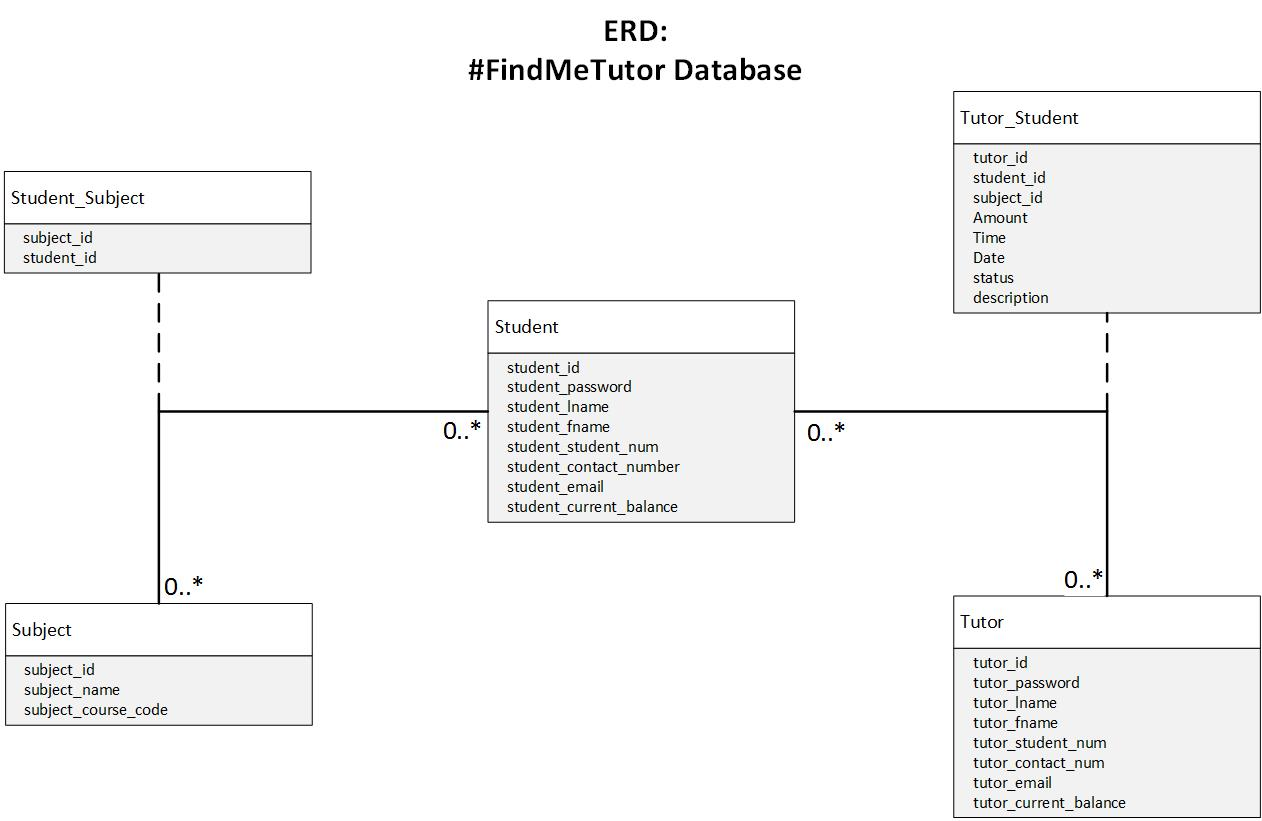
\includegraphics[width=140mm]{./class_diagram_findme_tutor.jpg}
%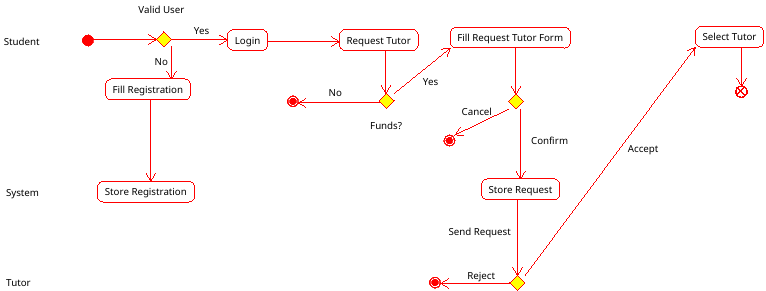
\includegraphics[width=140mm]{./activitydiagram.png}
%\includegraphics[width=140mm]{./.jpg}
\subsection{Development View}
Below is package diagrams of the FindMeTutor system:\\
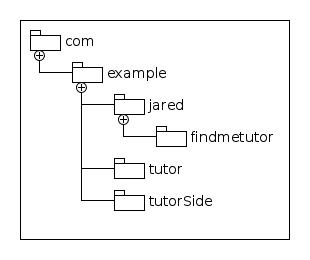
\includegraphics[width=140mm]{./Pakage.jpg}
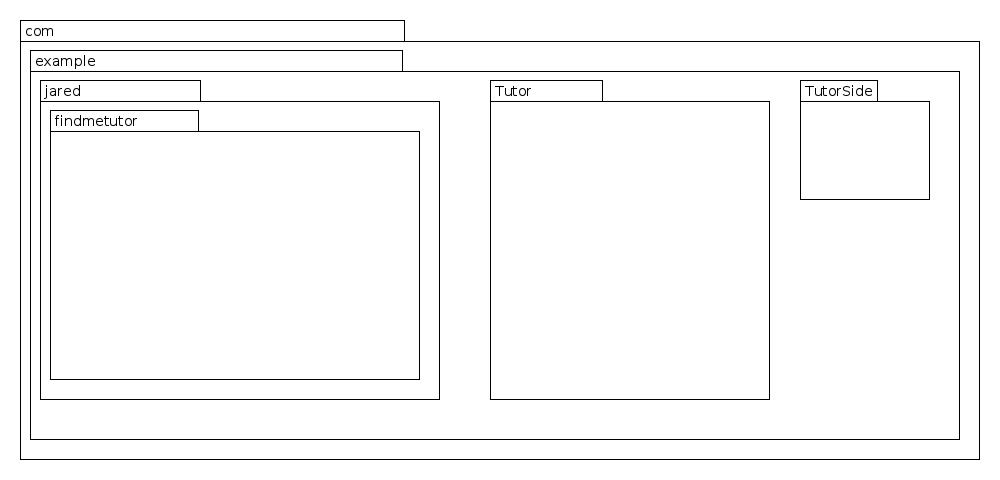
\includegraphics[width=140mm]{./Pakage2.jpg}
\subsection{Process View}
Below is an activity diagram of the Request Tutor use case:\\
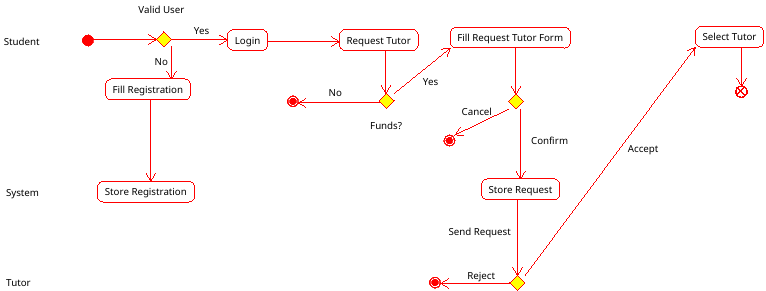
\includegraphics[width=140mm]{./activitydiagram.png}
\subsection{Physical View}
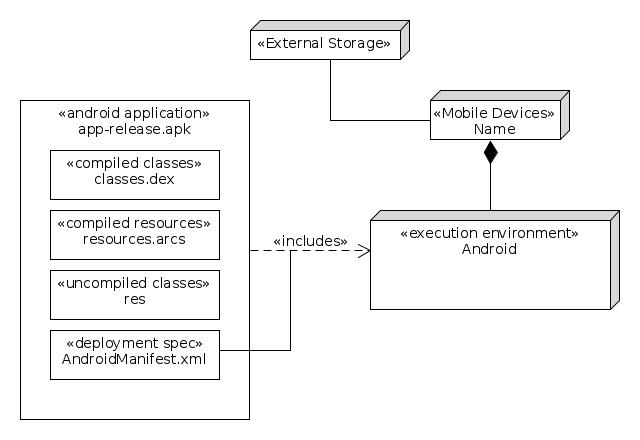
\includegraphics[width=140mm]{./Deployment.jpg}
\subsection{Scenarios}
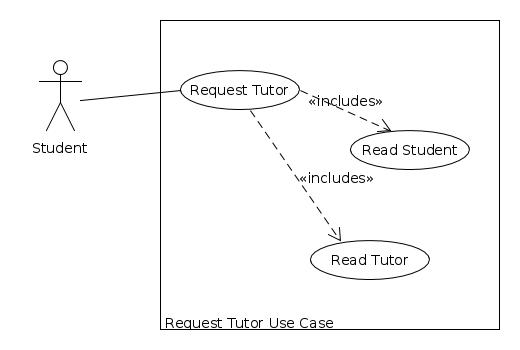
\includegraphics[width=140mm]{./RequestTutor.jpg}

\end{document}